\documentclass[]{fithesis3}
\usepackage[
	main=czech,
	english
]{babel}

\thesissetup{
    date          = \the\year/\the\month/\the\day,
    university    = mu,
    faculty       = fi,
    type          = bc,
    author        = Ondřej Přikryl,
    gender        = m,
    advisor       = {RNDr. Michal Procházka, Ph.D.},
    title         = {Integrace RemSig do klientských aplikací},
    keywords      = {remsig, pkcs11, csp, oauth2.0, ...},
}

\begin{document}
\chapter{Úvod}

Prvky informačních technologií se stávají každodenní součástí života a většina lidí by si bez nich již nedokázala život představit. Informační technologie uživatelům v mnoha směrech usnadňují život. Slouží jak k práci, tak i ke komunikaci se známými, zábavě a mnoha dalším činnostem. S rozšířením se však zvyšuje i potenciální riziko, které zneužití těchto prvků přináší. V době, kdy internet poskytuje základní komunikaci mezi více než miliardou lidí a je čím dál tím více používán jako nástroj k obchodování, se bezpečnost stává nesmírně důležitou otázkou, která by neměla zůstat nepovšimnuta. Částečnou odpovědí na tuto otázku bylo zavedení kryptografických systémů. I ty však nenabízí řešení ve všech případech a lidé by si měli stále dávat velký pozor. 

Kryptografie nebyla původní součástí návrhu internetu, ale v posledních dekádách se díky rozmachu digitálních technologií stala důležitým prvkem internetové infrastruktury. Přestože je skryta před zraky laických uživatelů, jde o důležitý vědní obor, který v současnosti prožívá obrovský posun kupředu. Tento vývoj je způsoben zejména tím, že si uživatelé začínají uvědomovat potřebu chránit své data a soukromí i ve virtuálním světě. Moderní kryptografie má mnoho podob a odvětví, jednou z nich je digitální podpis (též nazýván elektronický podpis), který je nezbytnou součástí systému RemSig.

Systém RemSig je bezpečné vzdálené úložiště certifikátů a privátních klíčů, které uživatelům poskytuje možnost podepisovat dokumenty bez nutnosti neustálého fyzického přístupu k zařízení, na němž je certifikát uložen. Důležitou součástí systému RemSig je uživatelská přívětivost. V současné době je systém možné používat pouze z webového rozhraní INET
\footnote{\url{https://inet.muni.cz}} 
a IS MU
\footnote{\url{https://is.muni.cz}}
, a proto je nutná implementace knihoven, které integrují funkce RemSigu do klientských aplikací. Náplní mé bakalářské práce je tyto knihovny implementovat a popsat základní prvky CSP a PKCS\#11. 


TODO popis struktury práce
%V první fázi práce se zaměřuji na vytvoření knihovny v programovacím jazyce C. Tato knihovna %obsahuje základní funkce pro práci s úložištěm certifikátů v operačním systému Windows pomocí %vývojového prostředí Cryptography API: Next Generation3 (dále CNG). V druhé fázi je zapotřebí %vytvořit knihovnu poskytující komunikaci mezi klientem a serverem a pomocí otevřeného %protokolu OAuth 2.0 získat přístup k datům uloženým na serveru RemSig. V poslední fázi spojuji již %implementované knihovny do fungujícího celku.

Výsledkem mé bakalářské práce jsou knihovny propojující RemSig a klientské aplikace . Důsledkem toho již není zapotřebí používat webové rozhraní INET a IS MU, což zaměstnancům MU výrazně usnadní práci při podepisování digitálních dokumentů. Nezávislost systému na webovém rozhraní univerzity také umožňuje jeho rozšíření mimo univerzitní kruhy.


\chapter{Digitální podpis}

Digitální podpis slouží k nahrazení obyčejného podpisu v digitálním světě. Je založen na asymetrické kryptografii a k jeho použití je zapotřebí dvojice klíčů - soukromého a veřejného. Digitální podpis zaručuje následující vlastnosti:
\begin{itemize}
\item Autenticitu - každý podpis je jednoznačně spojen s uživatelskou entitou, kterou může být jak běžný uživatel, tak i organizace nebo státní útvar (digitální značka).
\item Integritu dat - zaručuje, že data nebyla po cestě pozměněna. To je velice důležité k ujištění, že data, která byla odeslána, druhá strana také přijala.
\item Nepopiratelnost - autor nemůže popřít, že data nepodepsal. To je zajištěno tím, že k vytvoření podpisu je zapotřebí soukromý klíč, který má vlastník podpisu v držení a není veřejně znám.
\end{itemize} 
\section{Princip použití}
Uživatel si vytvoří dvojici klíčů, veřejný a soukromý. Soukromý klíč si ponechá a veřejný nechá potvrdit certifikační autoritou a následně jej zvěřejní. Podepsaný veřejný klíč nazýváme ceritifát. Podpis dokumentu poté probíhá následovně:
\begin{itemize}
\item uživatel spočítá haš (ang. hash) dokumentu - například pomocí rychlé hašovací funkce SHA256
\item haš zašifruje svým soukromým klíčem - například pomocí algoritmu RSA
\item data poté odešle společně s certifikátem a zašifrovaným hašem
\end{itemize}
Ověřování podpisu probíhá analogicky:
\begin{itemize}
\item osoba provádějící ověření spočítá haš dokumentu
\item za pomoci veřejného klíče osoby která dokument podepsala dešifruje přijatý digitální podpis a ověří, že získaný haš je shodný s vypočteným hašem
\end{itemize}
\begin{figure}[!ht]
  	\begin{minipage}{1.00\textwidth}
    		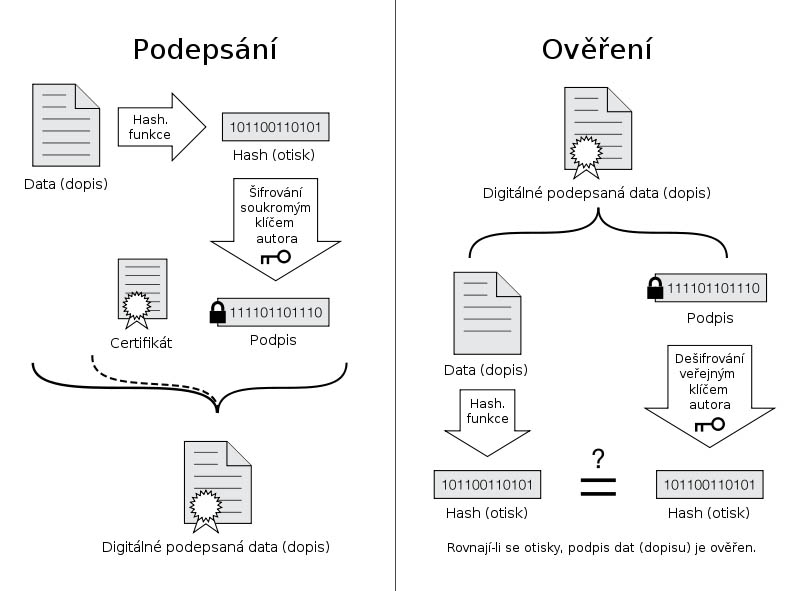
\includegraphics[width=\textwidth]{/home/oprikryl/Skola/bakalarka/obrazky/podpis.jpg}
  	\end{minipage}
 	\caption{Principy digitálního podpisu.}
  	\label{fig:Digitální podpis.}
\end{figure}
Pokud si haše odpovídají, pak je jisté, že přijatý dokument je shodný s odeslaným a je tedy zaručena integrita. Aby byla zajištěna nepopiratelnost a autenticita je nutné ověřit, že daný klíč opravdu patří osobě, která poslala podepsaný dokument. Procesu, který toto zajišťuje se říká \textit{přenos důvěry}.

\section{Přenos důvěry}
Aby bylo možné pomocí digitálního podpisu dosáhnout autenticity a nepopiratelnosti, je veřejný klíč dané osoby podepsán důvěryhodnou certifikační autoritou. Tímto způsobem je vyjádřeno, že certifikační autorita věří, že majitel veřejného klíče je skutečně ten za koho se vydává. Uživatel musí certifikační autoritě prokázat svoji totožnost předtím, než získá certifikát.
Další možností k dosažení auntenticity je tzv. \textit{síť důvěry}. Jedná se o decentralizovanou alternativu k centralizovanému modelu certifikačních autorit. 

\chapter{RemSig}

Systém RemSig je bezpečné vzdálené úložiště certifikátů a privátních klíčů, které uživatelům poskytuje možnost podepisovat dokumenty bez nutnosti neustálého fyzického přístupu k zařízení, na němž je certifikát uložen. Díky tomu odpadá uživatelům systému RemSig povinnost nosit s sebou hardwarové zařízení, což zvyšuje uživatelskou přívětivost i funkcionalitu. Uživatelé totiž mohou podepisovat dokumenty, i když u sebe právě nemají token, nebo když jsou na jiném počítači, který není nakonfigurovaný pro práci s digitálními podpisy nebo není důvěryhodný.

	\section{Aktuální využití}

		RemSig umožňuje podepisování dokumentů přímo z webového rozhraní systému INET
		a IS MU a je v souladu se současnou českou legislativou. RemSig je napojen na služby 				certifikační autority PostSignum
	\footnote{Kvalifikovaná certifikační autorita České Republiky, viz. \url{www.postsignum.cz/}}, 			což je další výhodou pro zaměstnance MU, kteří tak nemusí řešit vydání certifikátu třetí 			stranou, ale vše si pohodlně nastaví v rozhraní INET. Aktuálně je používána verze 					implementovaná v jazyce PHP, ale k dispozici je již nová verze implementovaná v jazyce 			Java, která již brzy nahradí starou implementaci. 
	
	\section{Autorizace} 

	Pro přístup k API systému je zapotřebí, aby se uživatel autentizoval klientovi, který 				zprostředkovává komunikaci mezi uživatelem a veřejně přístupnou API RemSigu.  
	\begin{figure}[!h]
  	\begin{minipage}{1.00\textwidth}
    		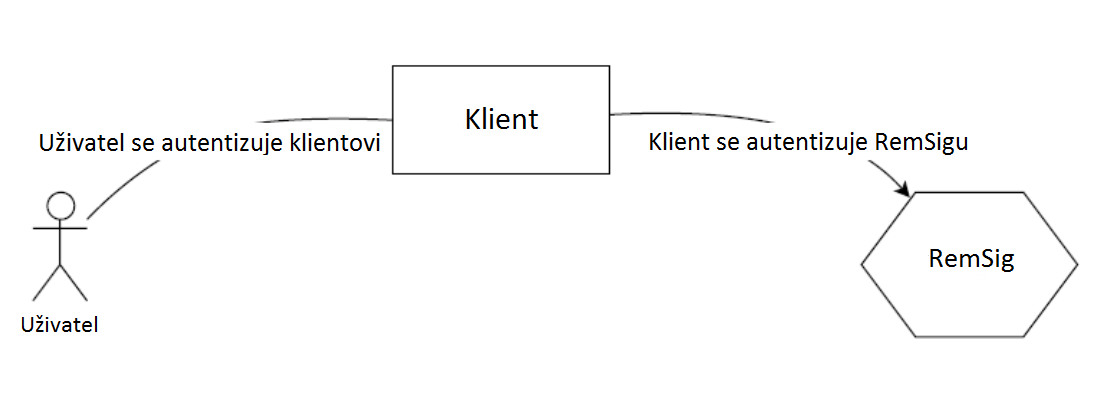
\includegraphics[width=\textwidth]{/home/oprikryl/Skola/bakalarka/obrazky/RemSigAten.png}
  	\end{minipage}
 	\caption{RemSig - Autentizace pomocí klienta.}
  	\label{fig:RemSig - Autentizace pomocí klienta.}
	\end{figure}
	Po autentizaci uživatele, Remsig obdrží od klienta unikátní identifikátor, podle kterého určí, ke 		kterým operacím je klient autorizován. Jestliže se identifikátor nenachází v seznamu pro řízení 		přístupu (ACL - Access Control List)
	\footnote{viz. \url{https://cs.wikipedia.org/wiki/Access_control_list}} , klient není oprávněn k 		žádné operaci.

		\subsection{Autentizace certifikátem}

		V nové verzi je podporována autentizace certifikátem. Poté, co se uživatel autentizuje 				klientovi, klient odešle RemSigu certifikát, pomocí kterého RemSig určí, ke kterým 				operacím je klient oprávněn. Tento přístup však není vyhovovující v případech, kdy chce 			klient komunikovat přímo s RemSigem. K tomu slouží protokol OpenID Connect.

		\subsection{OpenID Connect}

		OpenID Connect je již třetí verzí protokolu OpenID. Jedná se o protokol sloužící k 					ověřování identit, který staví na protokolu OAuth 2.0.  OpenID Connect umožňuje 				klientovi ověřit identitu koncového uživatele a získat základní informace o profilu. 					Podrobnému popisu protokolu OAuth 2.0 je věnována vlastní kapitola.

	\section{Role} 	
	Po úspěšné autentizaci získá klient přístup k metodám odpovídajícím jeho roli. RemSig rozlišuje 		dva typy rolí:
	\begin{itemize}
		\item Signer - podepisující
		\item Manager - manažer
	\end{itemize}
	\newpage
	Uživatelé systému IS MU mají roli podeposijícího. Ten má přístup k následujícím operacím:
	\begin{itemize}
		\item \textit{sign} - podepíše data podle defaultních kryptografických mechanismů
		\item \textit{signPKCS7} - vytvoří PKCS\#7
			\footnote{viz. \url{http://www.emc.com/emc-plus/rsa-labs/standards-initiatives/pkcs-7-cryptographic-message-syntax-standar.htm}} podpis dat
		\item \textit{signPdf} - slouží k podepisování PDF dokumentů
	\end{itemize}
	Zatímco manažer má přístup k následujícím operacím:
	\begin{itemize}
		\item \textit{importCertificate} - importuje certifikát do systému RemSig
		\item \textit{importPKCS12} - importuje strukturu dle standardu PKCS\#12
		\footnote{viz. \url{http://www.emc.com/emc-plus/rsa-labs/standards-initiatives/pkcs12-personal-information-exchange-syntax-standard.htm}}
		\item \textit{exportPKCS12} - exportuje soukromý klíč a certifikát ve struktuře 					definované standardem PKCS\#12
		\item \textit{changePassword} - změní heslo, kterým je chráněn soukromý klíč
		\item \textit{changeCertificateStatus} - změní status certifikátu
		\item \textit{listCertificates} - vypíše všechny certifikáty uložené v systému RemSig pro 			danného uživatele
		\item \textit{checkPassword} - zjistí, zda-li poskytnuté heslo skutečně slouží pro 					odemknutí privátního klíče
	\end{itemize}

	\section{Funkcionalita}
	Volání metod probíhá pomocí veřejně dostupné API. Při požadavku se klient musí autentizovat 		pomocí přístupového tokenu nebo certifikátu. Parametry a data jsou posílány formou XML 			dokumentu pomocí metody HTTP POST. Data odeslána RemSigu na podpis musí být 				kódována metodou BASE64\footnote{viz. \url{https://cs.wikipedia.org/wiki/Base64}}, přijatá 		data jsou také kódována pomocí BASE64. Kvůli 	bezpečnosti je použit protokol HTTPS.

		\begin{figure}[!ht]
  			\begin{minipage}{1.00\textwidth}
    			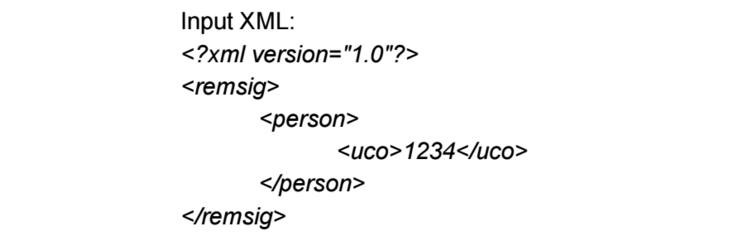
\includegraphics[width=\textwidth]{/home/oprikryl/Skola/bakalarka/obrazky/xml_input.png}
  			\end{minipage}
 			\caption{Ukázka XML požadavku metody \textit{listCertificates}.}
  			\label{fig:Ukázka XML požadavku.}
		\end{figure}

		\begin{figure}[!ht]
  			\begin{minipage}{1.00\textwidth}
    			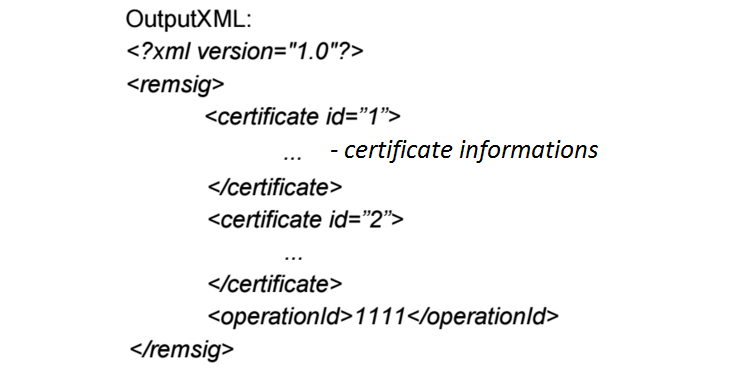
\includegraphics[width=\textwidth]{/home/oprikryl/Skola/bakalarka/obrazky/xml_output.png}
  			\end{minipage}
 			\caption{Ukázka XML odpovědi metody \textit{listCertificates}.}
  			\label{fig:Ukázka XML odpovědi.}
		\end{figure}

	\subsection{Správa úložiště}
	
	Aby uživatel mohl používat systém RemSig, musí v něm mít uložen certifikát a soukromý klíč. 		Remsig umožňuje generování dvojice soukromého a veřejného klíče přímo v systému. Po 			vygenerování je soukromý klíč zašifrován pomocí přiloženého PINu, který si uživatel sám zvolí. 		Dvojice je poté uložena do úložiště a klientovi je nazpět zaslán veřejný klíč, který je potřeba 		podepsat certifikační autoritou. Podepsaný certifikát je nutno opět odeslat systému. Uživatel 		však nemusí použít systém pro generování nové dvojice, ale může importovat již existující 			dvojici ve struktuře PKCS\#12 do systému.

	\begin{itemize}
	\item Import certifikátu 

		Metoda \textit{importCertificate} slouží k importování certifikátu do úložiště. Certifikát 			musí být ve formátu PEM. Tato metoda je používána v případě, kdy byla dvojice klíčů 				vygenerována systémem RemSig a veřejný klíč byl předán na podepsání certifikační 				autoritou.

	\item Import struktury PKCS\#12

		Metoda \textit{importPKCS12} slouží k nahrání dvojice vytvořené mimo systém RemSig. 			Tato dvojice je uložena ve struktuře PKCS\#12, která je zabezpečena heslem. Poté, co 			uživatel zadá heslo, je ze struktury exportována dvojice a uložena do úložiště RemSig. 				Uživatel musí poskytnout nové heslo, kterým bude zašifrován soukromý klíč.

	\item Export struktury PKCS\#12

		Metoda \textit{exportPKCS12} slouží k exportování dvojice ze systému RemSig. Jedinou 			možností jak exportovat certifikát a soukromý klíč je vytvořením PKCS\#12 struktury, do 		které je po zadání uživatelova PINu k soukromému klíči uložen certifikát a dešifrovaný 				soukromý klíč. Celá struktura je posléze zamknuta heslem.
	\end{itemize}

	\subsection{Podepisování dat}

	Jestliže má uživatel k dispozici certifikát a soukromý klíč, může začít používat metody 				vzdáleného podpisu. RemSig má k dispozici 3 metody na podepisování dat.

	\begin{itemize}
	\item Defaultní podpis
		
		Metoda \textit{sign} slouží k podpisu dat. K podpisu je použit defaultní kryptografický 				mechanismus. 
	
	\item PKCS\#7 podpis

		Digitální podpisy se od sebe mohou lišit v použitých algoritmech, ve formátu výstupu a v 			tom, zda-li výsledný podpis má být přiložen k datům či má být obdržen samostatně. 		

		Metoda \textit{signPKCS7} umožňuje nastavit tyto hodnoty a vytvořit podpis dle 					standardu PKCS\#7. Systém RemSig používá k nastavení těchto hodnot tzv. 						\textit{prifily}.

		Profily \newline
		Jestliže má organizace specifické požadavky na PKCS\#7 podpis, může si vytvořit profil, ve 		kterém si nastaví požadované hodnoty. Při vytváření nového profilu musí být nastaveny 			následující atributy:

		\begin{itemize}
		\item algorithm - algoritmus, který bude použit k podpisu
		\item no-detach - určuje, zda-li bude podpis přiložen k datům
		\item encoding - určuje formát výstupu
		\end{itemize}

		\begin{figure}[!h]
  			\begin{minipage}{1.00\textwidth}
    			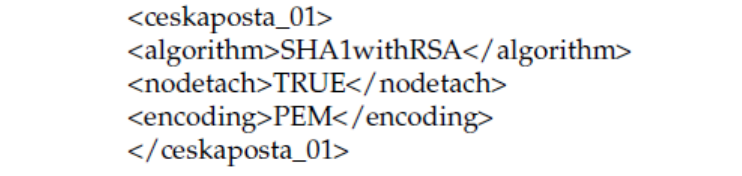
\includegraphics[width=\textwidth]{/home/oprikryl/Skola/bakalarka/obrazky/profile_ceskaposta.png}
  			\end{minipage}
 			\caption{Profil české pošty.}
  			\label{fig:Profil české pošty.}
		\end{figure}

		Na obrázku je uveden profil české pošty s označením jedna. Metoda s tímto profilem 				použije k vytvoření haše dat algoritmus SHA1 a výsledný haš zašifruje pomocí algoritmu 			RSA, podpis bude přiložen společně s daty a výstup bude ve formátu PEM.

	\item Podpis PDF dokumentu

	Pro podepisování PDF dokumentů slouží metoda \textit{signPdf}. Uživatel si zde může zvolit, 		zda bude vložen vodoznak do dokumentu či ne. K dispozici je již přednastavený vodoznak pro 		dokumenty MU. Uživatel si však může vytvořit vlastní nastavení, ve kterém je možné uvést 		pozici vodoznaku, stránky na kterých bude vodoznak umístěn, obrázek pozadí vodoznaku a 			text, který bude obsahovat.
	\end{itemize}	

\chapter{OAuth 2.0}

OAuth 2.0 (RFC 6749) je autorizační protokol (resp. framework), který umožňuje aplikacím třetích stran získat přístup ke službám HTTP, a to buď jménem registrovaného uživatele anebo jménem aplikace třetí strany. Protokol specifikuje pouze autentizaci klienta a výdej přístupového tokenu, přístup k jednotlivým zdrojům je již zcela nezávislý na protokolu. Je tedy zapotřebí veřejně dostupné API. Protokol OAuth 2.0 nahrazuje starý protokol OAuth 1.0 a není s ním zpětně kompatibilní.

	\section{Motivace}

	V tradičním modelu autentizace klient-server, žádá-li uživatel o přístup k zabezpečenému 			obsahu, je zapotřebí jeho autentizace pomocí přihlašovacích údajů. Aby tedy aplikace třetí 			strany mohla přistoupit k témuž obsahu, je zapotřebí s ní sdílet přihlašovací údaje oprávněné 		osoby. To však s sebou přináší několik problémů:

		\begin{itemize}
  		\item 
		Aplikace třetích stran si uchovávají přihlašovací údaje k budoucímu použití. Údaje bývají 			většinou uchovávány v otevřené podobě. Uchovávání pouze otisku je nedostatečné.

 		 \item 
		Uživatel ve většině případů nemůže omezit přístup aplikace k chráněnému obsahu, a to 			jak časovou platností, tak i omezením obsahu, ke kterému získá aplikace přístup.

 		 \item 
		Obvykle lze odebrat přístup aplikaci k zabezpečenému obsahu pouze 							změnou hesla. To se však projeví i u dalších aplikací, které jsou závislé na stejných 				přihlašovacích údajích.

  		\item 
		Kompromitace aplikace třetí strany znamená ohrožení přihlašovacích údajů 						uživatele a všech souborů na nich závislých.
		\end{itemize}

	OAuth tyto problémy řeší zavedením autorizační vrstvy a oddělením rolí klienta 					(aplikace) a vlastníka chráněného zdroje. V protokolu aplikace zažádá o přístup ke 				chráněnému obsahu  a jsou jí přiděleny přihlašovací údaje (přístupový token) odlišné od 			přihlašovacích údajů uživatele. 

	\section{Role}
		OAuth 2.0 definuje 4 typy rolí:

		\begin{itemize}
 		\item Vlastník zdrojů:
  		\newline
		Entita schopná přidělit přístup ke chráněnému obsahu. Jedná-li se o osobu, nazýváme ji 			koncový uživatel.
  		\item Server zdrojů:
  		\newline
		Poskytovatel a hostitel chráněného zdroje, schopný obsluhovat požadavky ke 					chráněnému zdroji pomocí přístupového tokenu.
 	 	\item Klient:
  		\newline
		Aplikace, která vyžaduje přístup ke chráněnému obsahu.
  		\item Server zdrojů:
 		\newline
		Server, který vydává klientovi přístupový token po úspěšné autentizaci oprávněné osoby.
		\end{itemize}
		Protokol nijak nespecifikuje interakci mezi autorizačním serverem a serverem zdrojů. 				Může se jednat o nezávislé entity, ale i o jeden server.

	\section{Přístupový token}	

	Pokaždé když klient potřebuje přistoupit k chráněnému obsahu, potřebuje přístupový token 			(anglicky \textit{access token}). Přístupový token je řetězec znaků, který opravňuje klienta k 		přístupu k chráněnému obsahu. V řetězci jsou skrytě uloženy informace o délce platnosti 			tokenu, o rozsahu přístupu k chráněnému obsahu a informace o vlastníkovi obsahu. Délka 			platnosti se může lišit implementací, ale typicky bývá platnost tokenu nastavena na 1 hodinu 		(3600 sekund).

	\section{Obnovující token}	

	Obnovující token (anglicky \textit{refresh token}) je získán společně s přístupovým tokenem a 		slouží k obnovení přístupového tokenu po vypršení jeho platnosti. Možnost získání 				přístupového tokenu pomocí obnovujícího tokenu bývá ve většině případech omezena počtem. 

	\section{Průběh protokolu}

	OAuth definuje několik základních způsobů autorizace vedoucích k získání přístupového 			tokenu. Patří mezi ně:

		\begin{itemize}
 		\item Autorizačním kódem:
  		\newline
		Jedná se o doporučený průběh, ke kterému je zapotřebí uživatelský agent 						(prohlížeč). Klient s použitím prohlížeče přesměruje uživatele na přihlašovací stránku. Po 			úspěšné autentizaci zašle autorizační server klientovi autorizační kód. Klient pro získání 			přístupového tokenu zašle autorizační kód autorizačnímu serveru.
  		\item Implicitně:
  		\newline
		Tento typ je zjednodušením průběhu autorizace autorizačním kódem. Slouží pro aplikace 			běžící v prohlížeči, které používají skriptovací jazyky jako je například JavaScript. Narozdíl 		od předchozího typu, klient získá přístupový token přímo po přihlášení. Tento typ je 				rychlejší,	jelikož redukuje počet výzev a odpovědí, které je potřeba udělat pro získání 				tokenu.
 	 	\item Zasláním přihlašovacích údajů:
  		\newline
		V tomto typu uživatel poskytne přihlašovací údaje klientovi. Klient zašle přihlašovací údaje 		autorizačnímu serveru, který po úspěšné autentizaci uživatele zašle zpět přístupový 				token. Přihlašovací údaje jsou použity jen pro získání přístupového a obnovujícího tokenu, 			není tedy potřeba jejich uložení pro budoucí použití. Tento typ je používán pouze při 				vysoké důvěře mezi uživatelem a aplikací. 
		\end{itemize}
		
	\newpage

	\section{Registrace klienta}

	Předtím než začne klient používat protokol, je potřeba jeho registrace na autorizačním serveru. 	Pro zvýšení bezpečnosti by klient měl poskytnout:

	\begin{itemize}
  		\item jeho typ - webová aplikace, nativní aplikace, zařízení
		\item adresu, na kterou bude token přesměrován
		\item jakoukoliv jinou informaci, kterou autorizační server požaduje (název, popis, smluvní 				podmínky, atd...).
	\end{itemize}

	Poté co se klient úspěšně zaregistruje, obdrží od autorizačního serveru unikátní identifikátor a 		heslo. Tyto údaje jsou nutné pro autentizaci klienta serveru během průběhu protokolu. Je-li při 		průběhu vyžadována adresa přesměrování, tak musí souhlasit s adresou uvedenou klientem při 	registraci.

	\begin{figure}[!ht]
  		\begin{minipage}{1.00\textwidth}
    			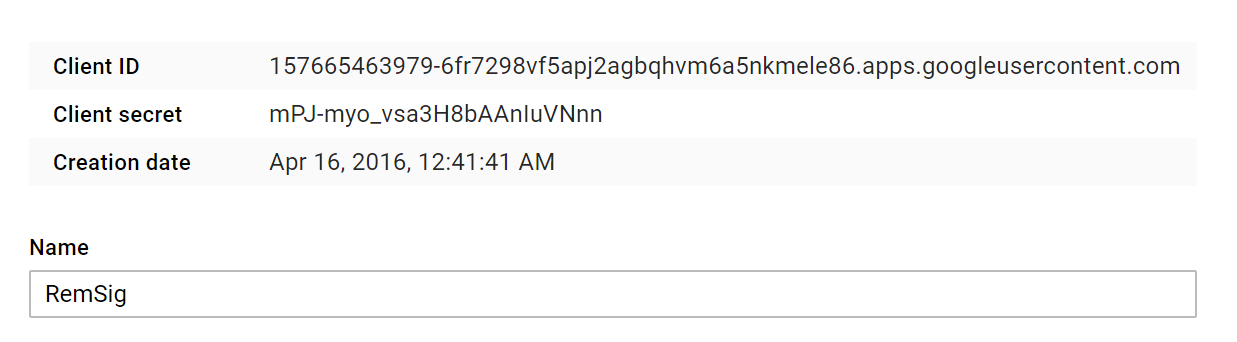
\includegraphics[width=\textwidth]{/home/oprikryl/Skola/bakalarka/obrazky/RemSigRegistration.png}
  		\end{minipage}
 		\caption{Google OAuth - registrace klienta.}
  		\label{fig:Google OAuth - registrace klienta.}
	\end{figure}	
	\newpage

\chapter{PKCS\#11}

S nástupem kryptografie přišla nutnost zavést jednotné protokoly a postupy pro zajištění kompatibility koncových aplikací. Ačkoliv se vývojáři shodli na základních kryptografických postupech, kompatibilita mezi jednotlivými implementacemi nebyla nikdy zaručena. Jednotný standard byl tedy nutností. Tuto potřebu naplnila organizace RSA Laboritories zavedením jednotného standardu Public-Key Cryptography Standards, zkráceně PKCS. Jedná se o celou rodinu standardů mezi které patří například i PKCS\#11, který je využit v implementaci knihoven RemSig.

PKCS\#11 je platformově nezávislé aplikační programové rozhraní (API) pro kryptografické tokeny, nazývané Cryptoki podle Cryptographic Token Interface. PKCS\#11 je nyní ve verzi 2.20 a to již od roku 2004. S ohledem na stáří protokolu probíhá od roku 2009 testování nové verze protokolu s označením 2.30, který však ještě nebyl standardizován.

	\section{Cíle návrhu}

	Cryptoki byl navržen s důrazem na jednotnost přístupu k rozdílným zařízením. Cílem rohraní je 		poskytnout vyšší aplikační vrstvě shodný přístup ke kryptografickému zařízení bez ohledu na 		konkrétní typ zařízení. Může se tak jednat o 
	Smart Card \footnote{viz. \url{https://cs.wikipedia.org/wiki/Smart_Card}} 
	, 
	PCMCIA \footnote{viz. \url{https://cs.wikipedia.org/wiki/PCMCIA}} 
	kartu nebo síťovou službu, aplikace využívající Cryptoki s nimi může pracovat bez ohledu na 		jejich hardwarovou odlišnost.

	Druhotným cílem bylo sdílení prostředků. S rozvojem víceúlohových operačních systémů se 		stalo žádoucím být schopen sdílet jedno zařízení mezi více aplikacemi. Stejně tak jedna 			aplikace by měla být schopna operovat s více kryptografickými zařízeními.

	\section{Model návrhu}

	Model použití Cryptoki začíná jednou nebo více aplikacemi, které požadují přístup k jednomu 		nebo více kryptografických zařízením. Tyto zařízení provedou operace požadované aplikací a 		vrátí výsledek.
	\begin{figure}[!ht]
  		\begin{minipage}{1.00\textwidth}
    			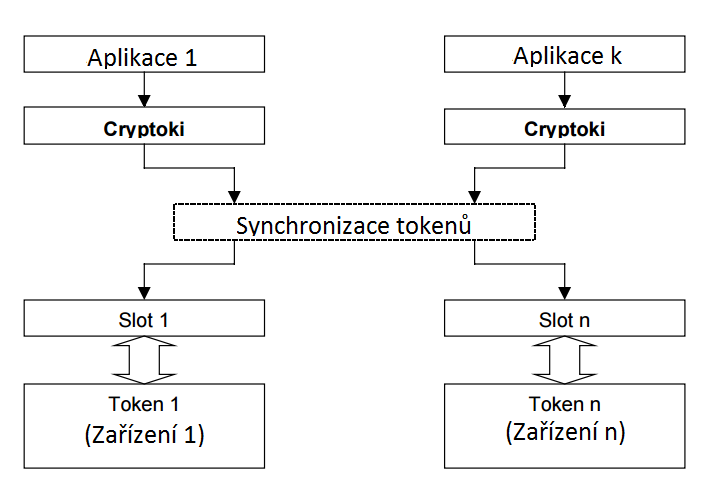
\includegraphics[width=\textwidth]{/home/oprikryl/Skola/bakalarka/obrazky/pkcs11_general_model.png}
  		\end{minipage}
 		\caption{PKCS11 - Obecný model.}
  		\label{fig:PKCS11 - Obecný model.}
	\end{figure}

	Cryptoki je tedy rozhraní mezi vyšší vrstvou uživatelských aplikací a nižší hardwarovou 			vrstvou, která vykonává kryptografické operace. Jak bylo popsáno výše, tato hardwarová 			vrstva může být reprezentována kartami, tokeny nebo dokonce vzdálenými síťovými službami.

	Díky tomu, že Cryptoki maskuje skutečnou hardwarovou podobu připojeného zařízení a 			zobrazuje je jako totožné jednotky, volající aplikace nemusí znát přesné rozhraní ke kterému je 		zařízení připojeno či jaký ovladač pro ně použít.

	Je nutné podotknout, že Cryptoki je pouze standard, nikoli knihovna. Tímto standardem je 			definované pouze rozhraní poskytované aplikacím, nikoliv podporované vlastnosti. Tyto se 			mohou lišit podle dané implementace a navíc standard nepředpisuje jaké vlastnosti mají být 			implementovány.

		\subsection{Objekty}

		Cryptoki vidí token jako zařízení, na kterém jsou uchovávány objekty a může vykonávat 			kryptografické operace. Cryptoki definuje 3 základní typy objektů:
		\begin{itemize}
			\item data - jsou definovány a spravovány aplikacemi
			\item certifikáty - uchovává certifikáty veřejného klíče
			\item klíče - uchovává kryptografické klíče
		\end{itemize}

		\begin{figure}[!ht]
  			\begin{minipage}{1.00\textwidth}
    				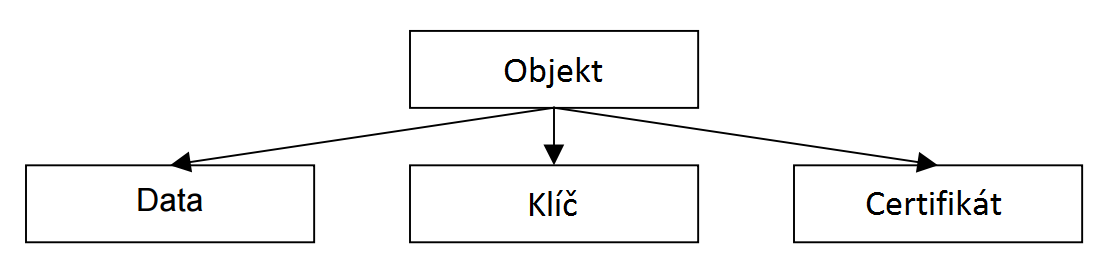
\includegraphics[width=\textwidth]{/home/oprikryl/Skola/bakalarka/obrazky/pkcs11_objekt.png}
  			\end{minipage}
 			\caption{PKCS11 - Objekty.}
  			\label{fig:PKCS11 - Objekty.}
		\end{figure}

		Objekty jsou zároveň klasifikovány dle jejich životnosti a viditelnosti. Podle životnosti jsou 			objekty rozděleny na \textit{session} a \textit{token} objekty. \textit{Token objekty} jsou 			objekty viditelné všem aplikacím připojeným k tokenu a jejich životnost není ovlivněna 				žádnou relací (tzn. setrvávají na tokenu dokud nejsou odstraněny). Zatímco 						\textit{session objekty} jsou viditelné pouze aplikaci, která je vytvořila a zanikají s 					ukončením relace.
		Objekty se dále mohou dělit na soukromé a veřejné. Pro přístup k veřejnému objektu se 			aplikace nemusí autentizovat tokenu, zatímco u soukromých je požadováno přihlášení 				pomocí PINu nebo jiné autentizační metody (např. biometrická zařízení).

		\newpage
		\subsection{Uživatelé}

		Cryptoki definuje dva typy uživatelů: 
		\begin{itemize}
			\item Security Officer (dále již jen SO) 
			\item normální uživatel
		\end{itemize}
		Oba vykonávají v systému různé úlohy, ale standard nedefinuje jejich vzájemný vztah. Je 			tedy v pořádku, když je stejná osoba normálnímm uživatelem i SO.

		Účelem SO je inicializovat token a nastavit normálnímu uživateli PIN nebo jinou formu 				autentizace. SO, na rozdíl od normálního uživatele, dokáže přistoupit pouze k veřejným 			objektům a nikoli k soukromým.

		Normální uživatel je jediný kdo může přistupovat k soukromým objektům, ale až poté co	
		se úspěšně autentizuje. Autentizace normálního uživatele může proběhnout až poté, co SO 		nastaví uživateli jeho PIN.

		\subsection{Relace}

		Pro práci s funkcemi a objekty tokenu je potřeba vytvořit alespoň jednu relaci (ang. 				\textit{session}). Jedná se o logické spojení, ve kterém aplikace komunikuje s tokenem. 			Relace se dělí na dva základní druhy:
		\begin{itemize}
			\item R/O relace (pouze pro čtení) 
			\item R/W relace (pro čtení i zápis).
		\end{itemize}

		R/W relace umožňují aplikaci číst, vytvářet, modifikovat a mazat objekty uložené na 				tokenu, zatímco R/O relace má přístup pouze ke čtení těchto objektů. Toto omezení se 				však vztahuje pouze na \textit{token objekty}, nikoliv na objekty vytvořené relací, ke 				kterým mají oba dva typy plný přístup. Po vytvoření relace má aplikace přístup pouze k 			veřejným objektům. Aby relace poskytovala přístup k soukromým objektům tokenu, je 				nutné aby se uživatel autentizoval tokenu. 

		Cryptoki umožňuje aplikacím vytvářet k jednomu tokenu více relací, ale zároveň také 				umožňuje tokenu omezit počet R/O a R/W relací, které může aplikace využít. Při zániku 			relace jsou odstraněny všechny \textit{session objekty} této relace a to i v případě, že 				jsou tyto objekty používány jinou relací.
		\newline
		\newline
		Stavy
		\newline
		Otevřená relace může být v jednom z pěti možných stavů. Tyto stavy definují, které 				objekty budou dostupné a jaké operace na nich budou povoleny. Pro R/O relace platí:

		\begin{itemize}
			\item R/O Public Session

			Aplikace si otevřela R/O relaci a doposud není autentizována tokenu. Aplikace má 					právo ke čtení veřejných \textit{token objektů} a právo ke čtení/zápisu veřejných 					\textit{session objektů}.
	
			\item R/O User Functions

			Aplikace si otevřela R/O relaci a uživatel se autentizoval tokenu. Aplikace má přístup 				ke čtení všech \textit{token objektů} a právo ke čtení/zápisu všech \textit{session 				objeků}.
		\end{itemize}

		\begin{figure}[!ht]
  			\begin{minipage}{1.00\textwidth}
    				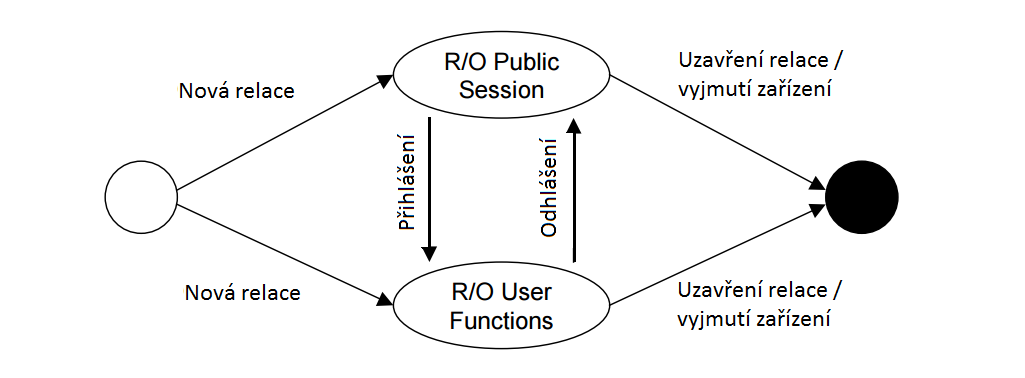
\includegraphics[width=\textwidth]{/home/oprikryl/Skola/bakalarka/obrazky/ro_sessions.png}
  			\end{minipage}
 			\caption{PKCS11 - Objekty.}
  			\label{fig:PKCS11 - Objekty.}
		\end{figure}

		\begin{itemize}
			\item R/W Public Session

			Aplikace si otevřela R/W relaci a doposud není autentizována tokenu. Aplikace má 				právo ke čtení/zápisu všech veřejných objektů.
	
			\item R/W User Functions

			Aplikace si otevřela R/W relaci a uživatel se autentizoval tokenu. Aplikace má přístup 			ke čtení/zápisu všech objektů.

			\item R/W SO Functions

			Aplikace si otevřela R/W relaci a SO se autentizoval tokenu. Aplikace má přístup 					pouze ke čtení/zápisu všech veřejných \textit{token objeků}. SO může nastavit PIN 				uživateli.
		\end{itemize}

		\begin{figure}[!ht]
  			\begin{minipage}{1.00\textwidth}
    				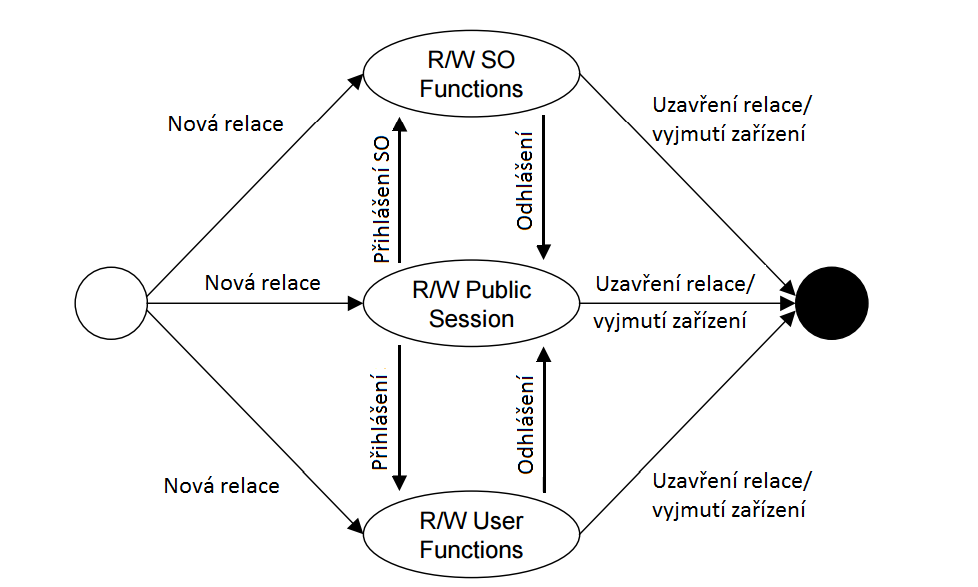
\includegraphics[width=\textwidth]{/home/oprikryl/Skola/bakalarka/obrazky/rw_sessions.png}
  			\end{minipage}
 			\caption{PKCS11 - Objekty.}
  			\label{fig:PKCS11 - Objekty.}
		\end{figure}	
		
\chapter{Praktická část}

	\section{OAuth 2.0}

	V praktické části jsem implementoval funkce standardního způsobu autorizace 					autorizačním kódem. Parametry jsou zasílané metodou POST.

	\begin{figure}[!ht]
		\begin{center}
  		\begin{minipage}{1.00\textwidth}
    			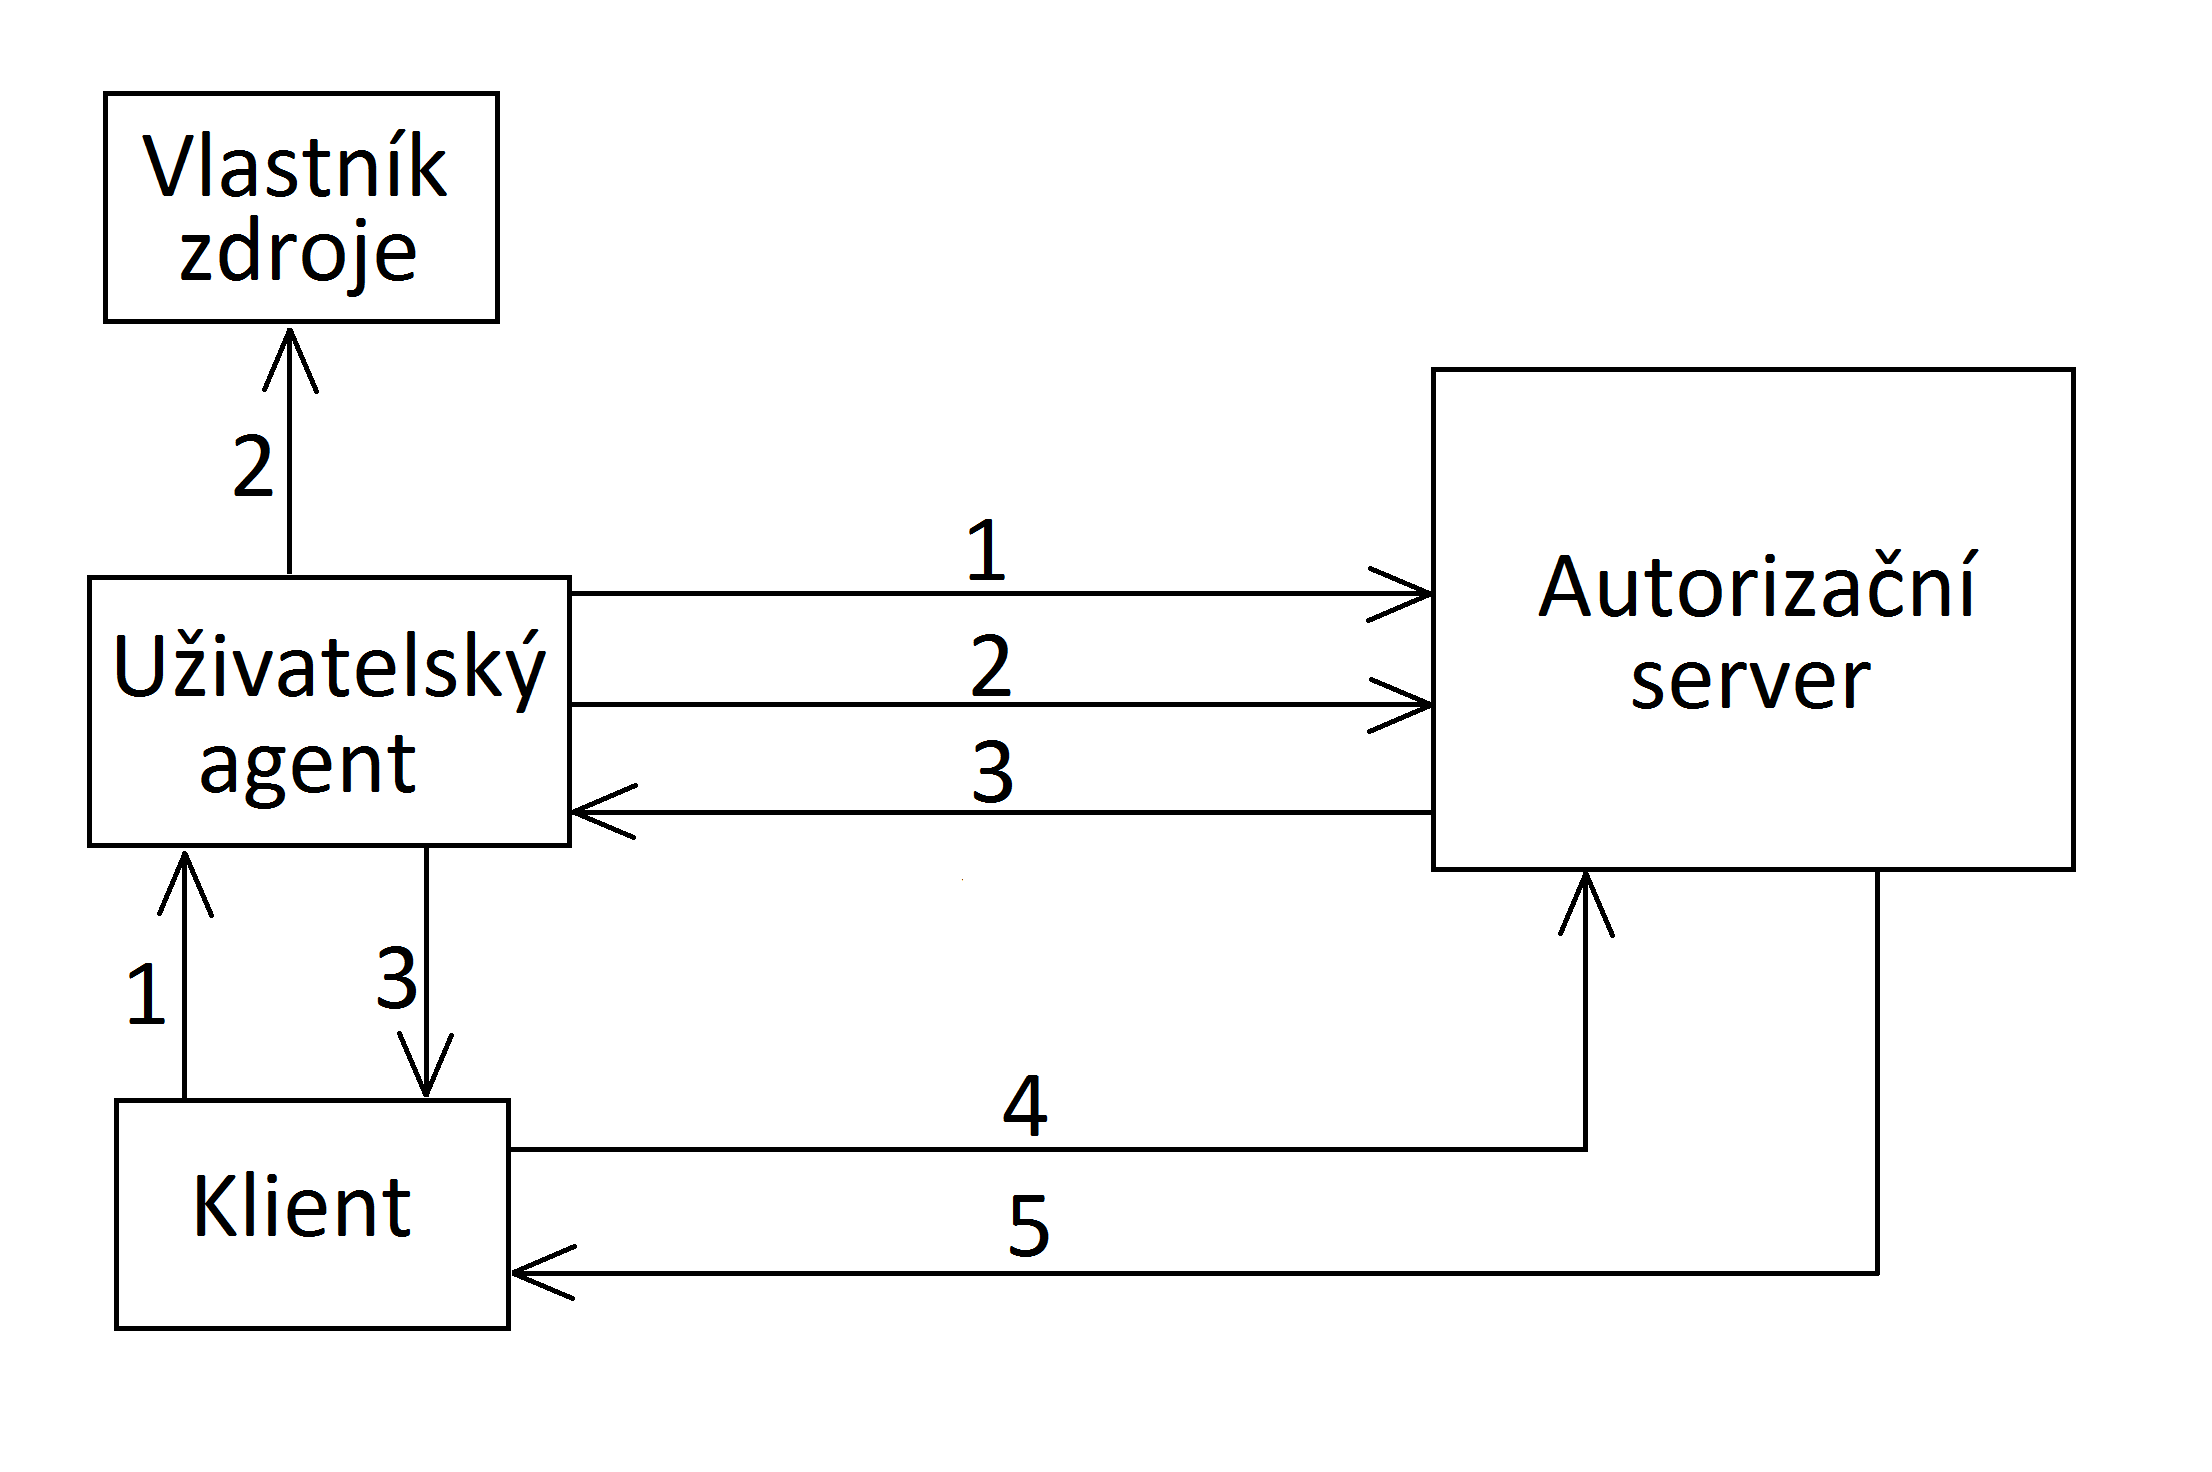
\includegraphics[width=\textwidth]{/home/oprikryl/Skola/bakalarka/obrazky/oauth.png}
  		\end{minipage}
		\end{center}
 		\caption{OAuth 2.0 - Autorizace autorizačním kódem.}
  		\label{fig:oauth}
	\end{figure}

	\begin{enumerate}
		\item {
		Klient pomocí prohlížeče přesměruje vlastníka zdroje na autorizační server. Klient v 				požadavku uvede svůj identifikátor, požadovaný rozsah přístupu,  identifikační řetězec
			\footnote {
			Identifikační řetězec (tzv. state) slouží k identifikaci sezení při větším počtu různých 				OAuth požadavků.
			}	 
		a adresu, na kterou má být zaslán autorizační kód.
		}
		\item
		Vlastník zdroje se autentizuje serveru a potvrdí klientovi přístup o daném rozsahu.
		\item
		Autorizační server přesměruje prohlížeč na adresu obdrženou v prvním kroku a předá jí 			autorizační kód a identifikační řetězec obdržený v prvním kroku.
		\item
		Klient zažádá autorizační server o přístupový token. V požadavku uvede autorizační kód 			přijatý v předchozím kroku, identifikátor klienta, příslušné heslo a adresu použitou k 				získání autorizačního kódu v prním kroku. 
		\item	
		Autorizační server zkontroluje identifikační údaje klienta a ověří platnost autorizačního 				kódu. Jestliže jsou všechny údaje platné, autorizační server zašle přístupový a obnovující 			token klientovi.

	\end{enumerate}

\end{document}